\subsection{Erweiterung des Nussinov-Algorithmus}

Der unspr\"ungliche Nussinov-Algorithmus bestimmt die maximal m\"ogliche Anzahl an Basenpaaren, die folgende Abwandlung bestimmt wie viele unterschiedliche Stukturen sind insgesamt m\"oglich sind.
\\\\
\textbf{Initialisierung:}
\begin{itemize}
	\item[] $Z(i,j)=1\ if\ i<j\le i+3$ 
	\item[] $Z(j+1, j) = 1$
\end{itemize}
\textbf{Berechnung:}
\begin{itemize}
	\item[]$Z(i,j)=+ \begin{cases}
               Z(i+1, j)\ (ungepaart)\\
               \displaystyle\sum_{i+3<k \le j}\ Z(i+1, k-1) * Z(k+1, j) * F(i,k)\\
\end{cases}$

	\item[] mit $F(i,k)= \begin{cases}
               1\ if\ i,k\ \epsilon\ \{AU, GC, GU\}\\
               -\infty\ else\\
\end{cases}$
\end{itemize}


\subsection{Zuker-Algorithmus}


In der Praxis ist der Nussinov-Algorithmus unzureichend, da eine Maximierung von Baasenpaaren nicht zwangsl\"aufig mit einer Maximierung von Stabilit\"at einhergeht. RNA's werden vorallem duch Interaktionen zwischen den Aromaten ihrer Basen stabilisiert. Das bedeutet, dass m\"oglichst lange Abschnitte von gepaarten Basen besonders stabil sind. Der Nussinov-Algorithmus maximiert lediglich die Anzahl der Basenpaare, ber\"ucksichtigt jedoch nicht wie die Basenpaare im Molkül verteilt sind. 
\\
Der Zuker-Algorithmus berechnet die optimale Sekundärstruktur einer RNA-Sequenz mit der minimalen freien Energie indem er thermodynamische Daten verwendet. Er geht davon aus, dass nicht die Struktur mit der maximalen Anzahl an Basenpaaren die stabilste Struktur darstellt, sondern jene mit der geringsten freien Energie. Dazu wird das RNA-Molek\"ul zunächst wie folgt nach dem Turner-Modell in einzelne Schleifen zerlegt.

\subsubsection{Turner-Modell (Nearest-Neighbor-Modell)}
Das Turner-Modell beschreibt die verschieden Untereinheiten/Schleifen eines RNA-Molek\"uls wie folgt:\\\\
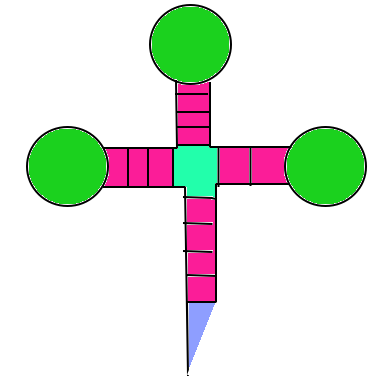
\includegraphics[scale=0.4]{lectures/160404_2/pix/turner}

\begin{itemize}
	\item 0 Basenpaare: exterior loop
	
\includegraphics[scale=0.4]{lectures/160404_2/pix/turner0}
	\item 1 Basenpaar: hair-pin loop
	
\includegraphics[scale=0.4]{lectures/160404_2/pix/turner1}
	\item 2 Basenpaare: interior loop
	
\includegraphics[scale=0.4]{lectures/160404_2/pix/turner2}
	
	\begin{itemize}
	\item 0 Basen ungepaart: stack\\
	
\includegraphics[scale=0.4]{lectures/160404_2/pix/stack}\\
	\item auf einer Seite eine Base ungepaart: buldge\\
	
\includegraphics[scale=0.4]{lectures/160404_2/pix/buldge1}\\
	\item auf beiden Seiten eine Base ungepaart\\
	
\includegraphics[scale=0.4]{lectures/160404_2/pix/buldge2}\\
	\end{itemize}
	
	\item $>$2 Basenpaare:  multi-loop
	
\includegraphics[scale=0.4]{lectures/160404_2/pix/turner3}
\end{itemize}

\subsubsection{Freie Energien}
Damit der Zuker-Algorithmus freie Energie minimieren kann, m\"ussen f\"ur die verschiedenen Basenkombinationen in den verschiedenen Loop-Arten Energiewerte gegeben sein. Diese wurden in aufwendingen Schmelztemperaturmessungen experimetell bestimmt. Es gibt Werte für alle m\"oglichen Stack-Arten und f\"ur alle Buldges und interior-Loops bis zu 2,3 Basenpaaren.\\\\
\paragraph{}
Die Energie eines Interior-Loops ist abh\"angig von:
\begin{itemize}
	\item den schließenden Basenpaaren
	\item den Basen, die den schließenden Basenpaaren benachbart sind
	\item der Anzahl der ungepaarten Basen
	\item der Assymetrie
\end{itemize}
\paragraph{}
Die Energie eines Hairpin-Loops ist abh\"angig von:
\begin{itemize}
	\item Typ der schließenden Basenpaaren
	\item den Basen, die den schließenden Basenpaaren direkt benachbart sind
	\item der Anzahl der ungepaarten Basen im Loop
\end{itemize}
\paragraph{}
Die Energie eines Multi-Loops ist abh\"angig von:
\begin{itemize}
	\item Anzahl der schließenden Basenpaaren
\end{itemize}

\subsubsection{Der Zuker-Algorithmus}
\begin{itemize}
\item[--]verwendet das Turner-Modell
\item[--]minimiert freie Energie: \textbf{minimum free energy} (mfe)
\item[--]Freie Energien sind additiv. Die Energie einer RNA-Struktur ist die Summe der freien Energien der einzelnen Schleifen.
\item[--]Festlegung: freie Energie der offenen Kette = 0
\end{itemize}
\paragraph{}
\textbf{Initialisierung:}
\begin{itemize}
	\item[] $F(i,j)=0\ if \ i<j\le i+3$ 
	\item[] $F(j+1, j) = 0$
\end{itemize}
\paragraph{}
\textbf{Berechnung:}
\begin{itemize}
	\item[]$F(i,j)=min \begin{cases}
               F(i+1, j)\ ($i$ ungepaart)\\
               \displaystyle\min_{i+3<k \le j}\ C(i,k) + F(k+1, j)\\
			\end{cases}$

	\item[] $C(i,j)= min \begin{cases}
               H(i,j)\\
               \displaystyle\min_{i<k<l<j}\ J(ij,kl) + C(k, l)\\
                \displaystyle\min_{i<u<l-5}\ M(i+1,u-1) + M^1(u, j-1) + a\\
                \end{cases}$
	\item[] $M(i,j)= min \begin{cases}
               M(i+1,j) + c\\
               \displaystyle\min_{i<k \le j}\ C(i,k) + b + (j-k)*c\\
                \displaystyle\min_{i<k<j-5}\ C(i,k) + b + M(k+1, j)\\
			\end{cases}$
	\item[]$M^1(i,j)= min \begin{cases}
               M^1(i,j-1) + c\\
              C(i,j) + b
			\end{cases}$
\end{itemize}
\paragraph{}
\begin{itemize}
	\item[]$a$ - Strafe f\"ur schließen eines Multi-Loops
	\item[]$b$ - Strafe f\"ur inneres Basenpaar in einem Multi-Loop
	\item[]$c$ - Strafe f\"ur ungepaarte Base in einem Multi-Loop
\end{itemize}
\paragraph{}
 \textbf{Grafische Darstellung des Zuker-Algorithmus}\\\\
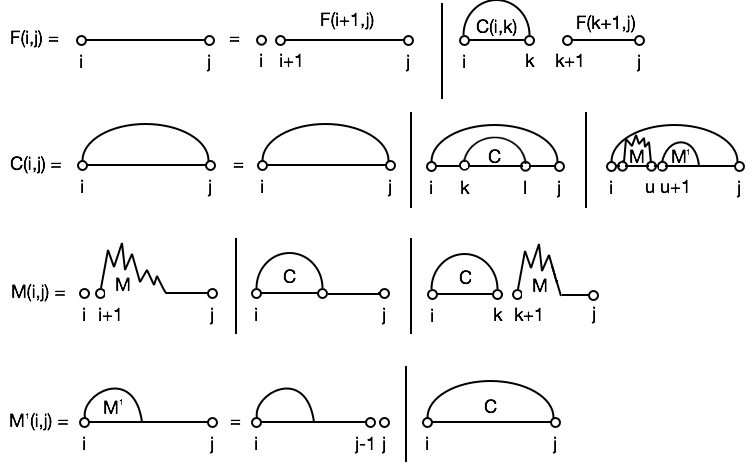
\includegraphics[scale=0.55]{lectures/160404_2/pix/zuker}
\paragraph{}
 \textbf{Komplexit\"at}
\begin{itemize}
	\item[] Speicher: $\mathcal{O}(n^2)$
	\item[] Prozessor: $\mathcal{O}(n^4)$
\end{itemize}
Um die Laufzeit einzuschr\"anken wird die Anzahl der ungepaarten Basen im Interior-Loop $j-l+k-i<$ Schwellenwert $\approx 30$.